\documentclass[12 pt]{beamer}
\usepackage[utf8]{inputenc}

\usepackage[]{amssymb}

\usepackage{multimedia}
\usepackage{media9}

\title{Geometric thickness of complete graphs}
\author{\normalsize{Manuel Gijón Agudo}}
%\date{10 July 2017}
\date{}

\mode<presentation>{\usetheme{Madrid}}
%\mode<presentation>{\usetheme[secheader]{Boadilla}}
\usecolortheme[ RGB={128,37,92} ]{structure}

\begin{document}

\begin{frame}[plain]
    \begin{center}

        Universidad Politécnica de Cataluña
        
        Facultad de Matemáticas y Estadística
        
        MAMMEE
        
        \scriptsize{Discrete and Algorithmic Geometry}
        
        \maketitle    
        M. Dillencourt, D. Eppstein, D. S, Hirschberg\\*
        
        \small{}
    \end{center}
    
    
\end{frame}

% DEFINICIONES DE COLORES
\setbeamercolor{amarilloNota}{bg=yellow!50!white}
\setbeamercolor{azulNota}{bg=blue!15!white}
\setbeamercolor{naranjaNota}{bg=orange!15!white}


% DIAPOSITIVA 0
\begin{frame}{0}
    \frametitle{Index}
     
    \tableofcontents  
\end{frame}

%%%%%%%%%%%%%%%%%%%%%%%%%%%%%%%%%%%%%%%%%%%%%%%%%%%%%%%%%%%%%%%%%%%%%%%%%%%%
\section{Motivation and first definitions}

% DIAPOSITIVA 1
\begin{frame}{1}
    \frametitle{An economic motivation}
    Suposse we have to print a circuit into a circuit board. Is more efficient to use uninsulated wires.
    
  
    \centering{
    \includegraphics[scale = 0.3]{"Circuit Board".jpg}
    }
    
    Problem: avoid dead shorts. Solution: separe the wires in different layers.
    This problem is equivalent to mimimize the number of layers.
    
\end{frame}

% DIAPOSITIVA 2
\begin{frame}{2}
    \frametitle{Improve the display of a graph}
    Now we imagine that we want to display information in a graph-shape.
    
    \centering{
    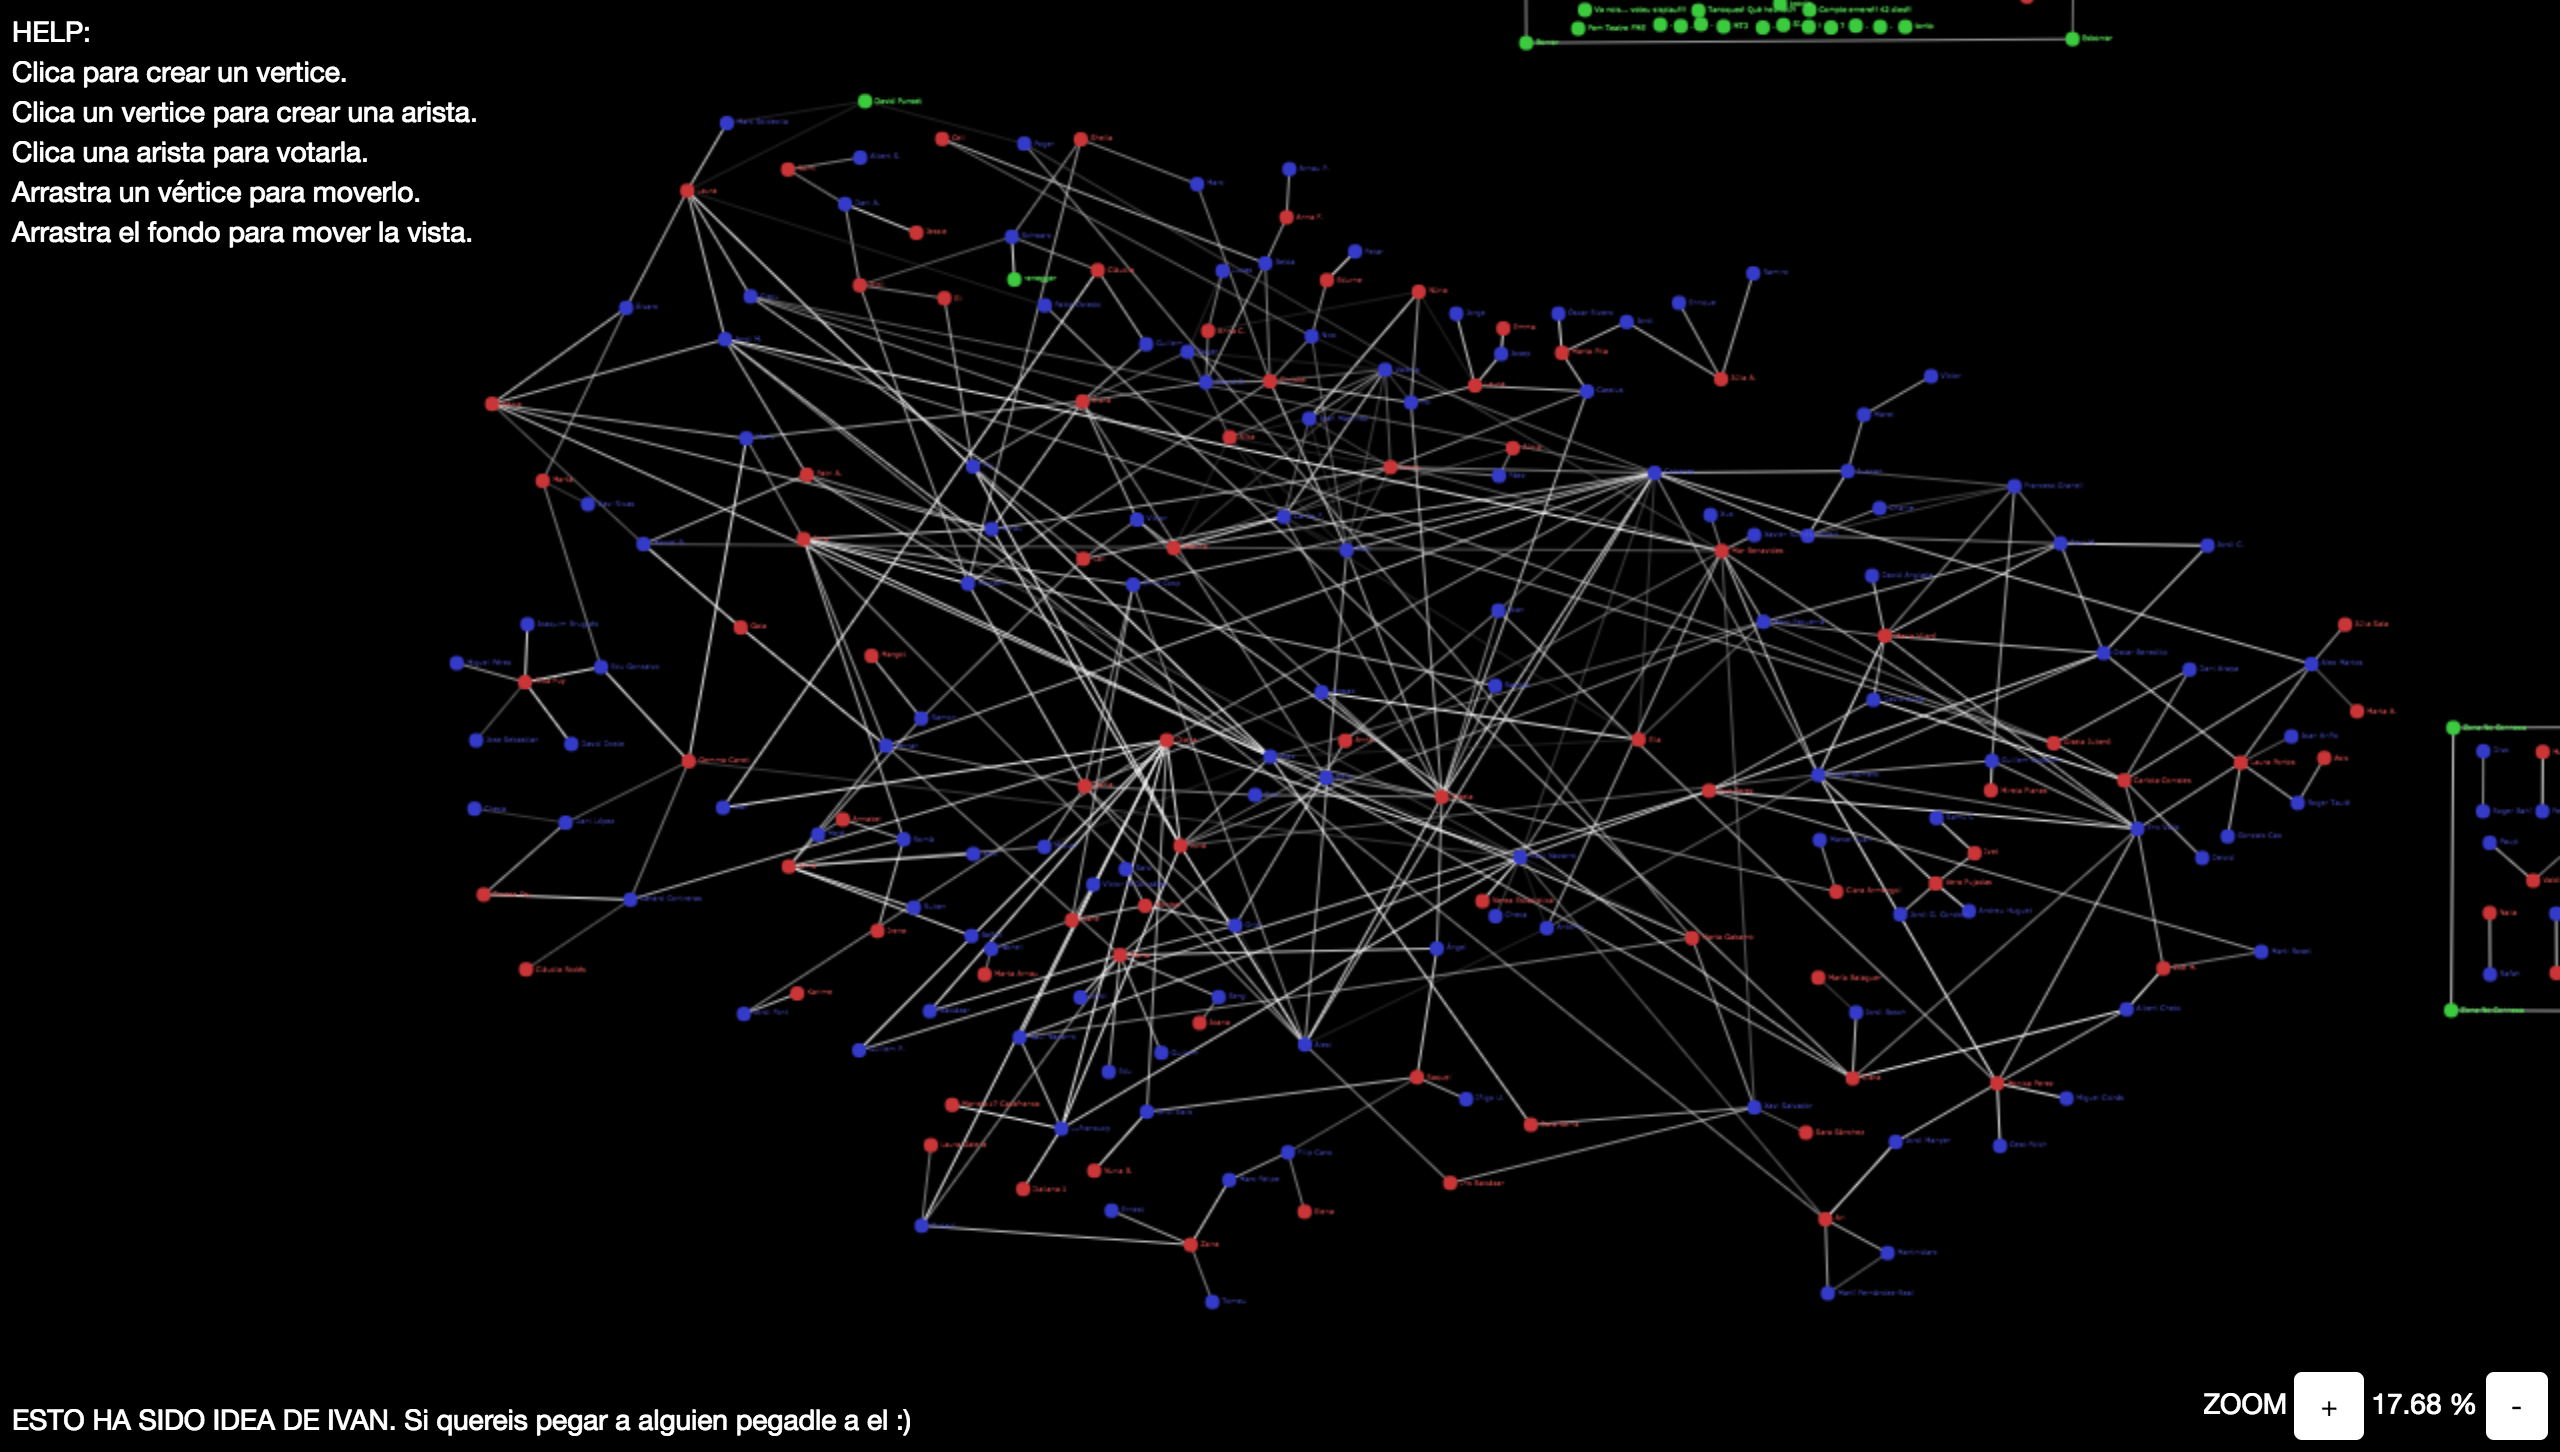
\includegraphics[scale = 0.2]{Grafo_FME.png}
    }

    The concept of the thickness of a graph is related with the number of colors we need to separate oll the edges.
    
\end{frame}

% DIAPOSITIVA 3
\begin{frame}{3}
    \frametitle{Thickness of a graph $\mathcal{G}$}
  
    \begin{block}{Theorical Thickness $\theta (\mathcal{G})$}
    Minimum number of planar graphs into a which a graph can be descomposed.
    \end{block}
    
    \pause
    
    \begin{block}{Geometric Thickness $\bar{\theta} (\mathcal{G})$}
    Smallest value of $k$ such that we can assign a planar point locations to the vertices of $\mathcal{G}$, represent each edge of $\mathcal{G}$ as a line segment, and assign each edge to one of $k$ layers so that no two edges on the same layer cross.
    \end{block}

\end{frame}

% DIAPOSITIVA 4
\begin{frame}{4}
    \frametitle{Thickness of a graph}
  
    \begin{alertblock}{Key difference}
    Geometric thickness requires that the vertex placements be consistent at all layers and that straight-line adges be used, whereas graph-theorical thickness imposes no consistency requirement between layers.
    \end{alertblock}
\end{frame}

%%%%%%%%%%%%%%%%%%%%%%%%%%%%%%%%%%%%%%%%%%%%%%%%%%%%%%%%%%%%%%%%%%%%%%%%%%%%
\section{Results}

    \subsection{Good news}

% DIAPOSITIVA 5.a
\begin{frame}{5}
    \frametitle{Graph-theorical thickness for all complete graphs}
    
    $$
    \boxed{
    \theta (\mathnormal{K}_{n}) = 
    \begin{cases}
    1, \quad 1 \leq n \leq 4\\
    2, \quad 5 \leq n \leq 8\\
    3, \quad 9 \leq n \leq 10\\
    \lceil \frac{n + 2}{6} \rceil, \quad n > 10\\
    \end{cases}
    }
    $$

\end{frame}

% DIAPOSITIVA 5.b
\begin{frame}{5}
    \frametitle{Graph-theorical thickness for all complete graphs}
    
    \centering
    \includegraphics[scale = 0.6]{"Geometrical-theorical thickness from 1 to 30".png}
    
\end{frame}

    \subsection{Upper and lower bounds}

% DIAPOSITIVA 6.a
\begin{frame}{}
    \frametitle{Upper Bounds}
    
    \begin{block}{\textbf{Theorem 1}}
    $$\bar{\theta} (k_{n}) \leq \lceil n/4 \rceil $$
    \end{block}
    
    \pause
    
    \textbf{Roadmap to the proof:}
    
    \begin{itemize}
        \item Assume that $n$ is multiple of four, $n = 2k$ with ($k$ even), show that $n$ vertices can be arranged in two ``rings'' of $k$ vertices, so $K_{n}$ can be embedded using $k/2$ layers and with no edges on the same layer crossing.
    \end{itemize}
\end{frame}

% DIAPOSITIVA 6.b
\begin{frame}{}
    \frametitle{Upper Bounds}

    \textbf{Roadmap to the proof:}
    
    \begin{itemize}
        \item Use the vertices of the inner ring to form a regular $k$-gon and considerer the opposite vertices con create a zigzag path. This path has exactly one diagonal connecting diametrically opposite points. 
        
        \item By continuity, we can replace by a suitably chosen common end points the infinite end points of a collection of parellel rays. Thus forming an outer ring of $k$ vertices.
        
        \item The figure can be perturbed by moving slightly the inner ring. None of the diagonals of the polygon comprinsing the outher ring intersect the polygon comprising the inner ring.
        
        \item It's straighforward to verify that this is indeed a descomposition of the edges of $k_n$ into $k/2 = n/4$ layers.
    \end{itemize}
    
    \begin{flushright}
    $\blacksquare$
    \end{flushright}
\end{frame}


% DIAPOSITIVA 7
\begin{frame}{}
    \frametitle{Lower Bounds}
    
    \begin{block}{\textbf{Theorem 2}} 
    For all $n \geq 1$
    $$\bar{\theta} (k_{n}) \geq \max_{1 \leq x \leq n/2} \frac{\binom{n}{2} - 2\binom{x}{2} - 3}{3n - 2x - 7}$$
    \end{block}
    
    \pause
    
    \begin{exampleblock}{In particular, for $n \geq 12$}
    $$
    \bar{\theta} (k_{n}) \geq \left \lceil \frac{3 - \sqrt{7}}{2}n + 0.342 \right \rceil  \geq \left \lceil \frac{n}{5.646} + 0.342 \right  \rceil 
    $$
    \end{exampleblock}
\end{frame}

    \subsection{$K_{15}$}
    
% DIAPOSITIVA 8.a
\begin{frame}{}
    \frametitle{Geometric Thickness of $K_{15}$}
    
    \begin{block}{\textbf{Theorem 3}}
    $$\bar{\theta} (k_{15}) = 4 $$
    \end{block}
    
    \pause
    
    \textbf{Proof:}
    We divide the proof in $3$ cases.
    
    \begin{itemize}
    \item \textbf{Case I:} $3$ points in the convex hull. 
    Let $\mathcal{A, B}$ and $\mathcal{C}$ convex hull points and let $\mathcal{A}_{1}, \mathcal{B}_{1}$ and $\mathcal{C}_{1}$ be the point furtherst from edge $\mathcal{BC}$ (respectively $\mathcal{AC}, \mathcal{AB}$ within triangle $\mathcal{ABC}$).
        \begin{itemize}
            \item \textbf{Lemma 1:} The edge $\mathcal{AA}_{1}$ will appear in every triangulation of $\mathcal{S}$.
        \end{itemize}
    Let $\mathcal{A}_{2}, \mathcal{B}_{2}$ and $\mathcal{C}_{2}$ be the point next furtherst from edge $\mathcal{BC}$ (respectively $\mathcal{AC}, \mathcal{AB}$ within triangle $\mathcal{ABC}$.
        \begin{itemize}
            \item \textbf{Lemma 2:} At least one of the edges $\mathcal{A}_{1}\mathcal{A}_{2}$ or $\mathcal{A}\mathcal{A}_{2}$ will appear in every triangulation of $\mathcal{S}$.
        \end{itemize}
    \end{itemize}
\end{frame} 

% DIAPOSITIVA 8.b
\begin{frame}{}
    \frametitle{Geometric Thickness of $K_{15}$}
    
    \begin{block}{\textbf{Theorem 3}}
    $$\bar{\theta} (k_{15}) = 4 $$
    \end{block}

    \textbf{Proof:}
    We divide the problem in $3$ cases.
    
    \begin{itemize}
    \item \textbf{Case II:} $4$ points in the convex hull. 
        \begin{itemize}
            \item Let $\mathcal{A, B, C, D}$ the convex hull vertices.
            \item Assume triangle $\mathcal{DAB}$ has at least one point of $\mathcal{S}$ in his interior (if not switch $\mathcal{A}$ and $\mathcal{C}$ and let $\mathcal{A}_{1}$ be the point inside furthest from line $\mathcal{DB}$).
            \item By Lemma 2, the edge $\mathcal{AA}_{1}$ must appear in every triangulation of $\mathcal{S}$.
            \item Since every triangulation has $38$ edges three triangulations can account at most $104$ edges.
        \end{itemize}
    \end{itemize}
\end{frame} 

% DIAPOSITIVA 8.c
\begin{frame}{}
    \frametitle{Geometric Thickness of $K_{15}$}
    
    \begin{block}{\textbf{Theorem 3}}
    $$\bar{\theta} (k_{15}) = 4 $$
    \end{block}

    \textbf{Proof:}
    We divide the problem in $3$ cases.
    
    \begin{itemize}
    \item \textbf{Case III:} $5$ or more points in the convex hull. 
        \begin{itemize}
            \item Let $h$ be the number of points in the convex hull.
            \item A triangulation of $\mathcal{S}$ will have $42 - h$ edges, and all hull edges must be in each triangulation.
            \item The total number of edges in three triangulatinos is at most $3(42 -  2h) + h = 126 - -5h$, that is at most $101$ for $h \geq 5$.
        \end{itemize}
    \end{itemize}
    
    \begin{flushright}
    $\blacksquare$
    \end{flushright}
\end{frame} 

    \subsection{Bipartite graphs}
    
% DIAPOSITIVA 9
\begin{frame}{}
    \frametitle{Geometric Thickness of Complete Bipartite Graphs}
    
    \begin{block}{\textbf{Theorem 4}}
    For the complete bipartite graph $K_{a, b}$
    $$\left \lceil \frac{ab}{2a + 2b - 4} \right \rceil \leq \theta (K_{a,b}) \leq \bar{\theta} (k_{a,b}) \leq \left \lceil \frac{\min(a, b)}{2}  \right \rceil$$
    \end{block}
    
    \pause
    
    \textbf{Proof:}
    \begin{itemize}
    \item First inequality: from Euler's formula since a bipartite graph which is planar with $a + b$ vertices can have at most $2a + 2b -4$ edges
    \item Second inequality: assume that $a \leq b$ and $a$ is even. Draw $b$ vertices in a horizontal line, with $a/2$ red vertives above the line and $a/2$ vertices below.
    Each layer consists of all edges connecting the blue vertices with one red vertex from above the line and one red vertex from below.
    \end{itemize}
    
    \begin{flushright}
    $\blacksquare$
    \end{flushright}
\end{frame}

% DIAPOSITIVA 10
\begin{frame}{}
    \frametitle{Geometric Thickness of Complete Bipartite Graphs}
    
    \begin{block}{\textbf{Corollary 1:}}
    For any integer $b$, $\bar{\theta} (k_{a,b}) = \theta (k_{a,b})$ provided:
    $$ a >
    \begin{cases}
    \frac{(b-2)^2}{2}  & \text{if b is even}\\
    (b-1)(b-2)  & \text{if b is odd}
    \end{cases}
    $$
    \end{block}
    
    \pause
    
    \textbf{Proof:}
    If $a > b$, the leftmost and rightmost quantities in the expresion of the last theorem will be equal provided $ab/(2a + 2b -4) > (b - 2)/2$ if $b$ is even, or provided  $ab/(2a + 2b -4) > (b - 1)/2$ f $b$ is odd. By simplifing this inequality holds.
    
    \begin{flushright}
    $\blacksquare$
    \end{flushright}
\end{frame}


% DIAPOSITIVA 11
\begin{frame}{}
    \frametitle{Geometric Thickness of Complete Bipartite Graphs}
    
    \begin{block}{\textbf{Theorem 5}}
    $$\bar{\theta} (k_{6,8}) = 3$$
    \end{block}
    
    \pause
    
    \textbf{Roadmap to the proof:}
    
    \begin{itemize}
    \item From the last theorem, second inequality: $\bar{\theta} (k_{6,8}) \leq 3$
    \item <2-> We need to show that $\bar{\theta} (k_{6,8}) > 2$. We proceed by contradiction: we have an embedding of $k_{6,8}$ with geometric thickness $2$ and underlying points set $\mahtcal{S}$.
    A graph with $14$ edges has at most $24$ edges (Euler), so each layer each layer has exactly $24$ edges.
    \end{itemize}
    \end{frame}

% DIAPOSITIVA 11.b
\begin{frame}{}
    \frametitle{Geometric Thickness of Complete Bipartite Graphs}
    
    \begin{block}{\textbf{Theorem 5}}
    $$\bar{\theta} (k_{6,8}) = 3$$
    \end{block}
    
    \textbf{Roadmap to the proof:}    
    
    \begin{itemize}
    \item We claim that must be at least one red and one blue vertex on the convex hull of $\mathcal{S}$. Again by contradriction, we suppose that all convex hull vertices are the same color.
    
        \begin{itemize}
            \item Use bipartition and the number of vertices in each layer.
            \item Contradiction! $\Rightarrow$ there are at least one red and one blue vertex.
        \end{itemize}
    \end{itemize}
\end{frame}
    
% DIAPOSITIVA 11.c
\begin{frame}{}
    
    \frametitle{Geometric Thickness of Complete Bipartite Graphs}
    
    \begin{block}{\textbf{Theorem 5}}
    $$\bar{\theta} (k_{6,8}) = 3$$
    \end{block}
    
    \textbf{Roadmap to the proof:}
    
    \begin{itemize}
        \item The claim implies that one of the layers must contain a convex hull edge.
        \item This edge could be added to the second layer without destroying planarity..
        \item Since the second layer has already $14$ vertices and $24$ edges it's imposible, which leads us to a contradiction. $\Rightarrow$ $\bar{\theta} (k_{6,8}) > 2$
    \end{itemize}
    \begin{flushright}
    $\blacksquare$
    \end{flushright}
\end{frame}

    \subsection{To sum up}
    
% DIAPOSITIVA 12.a
\begin{frame}{}
    \frametitle{The first 100 values of  $\bar{\theta}$}
    \centering{
    \includegraphics[scale = .6]{"Comparation".png}
    }
\end{frame}

% DIAPOSITIVA 12.b
\begin{frame}{}
    \frametitle{The first 100 values of  $\bar{\theta}$}
    \centering{
    \includegraphics[scale =.6]{"Known common values 2".png}
    }
\end{frame}

%%%%%%%%%%%%%%%%%%%%%%%%%%%%%%%%%%%%%%%%%%%%%%%%%%%%%%%%%%%%%%%%%%%%%%%%%%%%
\section{Conclusions and open questions}

% DIAPOSITIVA 13
\begin{frame}{}
    \frametitle{Some open questions}
    
    \begin{itemize}
        \item To find exact values for $\bar{\theta}(K_{n})$, in particular for $n = 13, 14$.
        \item What is the smallest graph $\mathcal(G)$ such that $\bar{\theta}(\mathcal{G}) > \theta(\mathcal{G})$?
        \item What is the complexity of computing $\bar{\theta}(\mathcal{G})$ for a given graph $\mathcal{G}$?.
    \end{itemize}
    
\end{frame}

%%%%%%%%%%%%%%%%%%%%%%%%%%%%%%%%%%%%%%%%%%%%%%%%%%%%%%%%%%%%%%%%%%%%%%%%%%%%
% DIAPOSITIVA FINAL
\begin{frame}{}
    \frametitle{Bibliography}
    
    
    \begin{thebibliography}{ABC9999}

    \bibitem[Ben]{Bens}
    D.Dillencourt, D. Eppstein and D.\,S. Hirschberg,
    \textit{Geometric thickness of complete graphs}, 
        J. Graph Algorithmss and Applications 4 (3), 5-17, 2000.
        %http://www.maths.abdn.ac.uk/∼bensondj/
	    
	\bibitem[PTM]{PTM}
    P. Mutzel, T. Odenthal, M. Scharbrodt, 
    \textit{The thickness og graphs: a survey}, 
        Graphs and Combinatorics, March 1998, Volume 14, Issue 1, pp 59–73.
    \end{thebibliography}
        
\end{frame}

\end{document}
